\documentclass{article}
\usepackage{fullpage}
\usepackage{graphicx}

\title{Aye-Aye Sleep Monitoring}
\author{Nathan Hui\\Engineers for Exploration\\UC San Diego\\nthui@ucsd.edu}
\begin{document}
\maketitle
\section{Introduction}
In 2020, the San Diego Zoo Wildlife Alliance\footnote{https://science.sandiegozoo.org/} and Engineers for Exploration\footnote{https://e4e.ucsd.edu} set on a path to develop a system for monitoring animals in the care of the San Diego Zoo, both at the Zoo in Balboa Park, the Safari Park in Escondido, and the Biodiversity Reserve behind the Safari Park.  The aim of this system was to provide 24/7 automated monitoring of animals with intelligent identification of abnormalities in behavior, which could indicate to animal care specialists the need to pay attention to certain things.  This system would also provide a corpus of data for future machine learning/artificial intelligence tools.

The first phase of this system was aimed at monitoring the aye-aye lemur (\textit{Daubentonia madagascariensis}) housed at the San Diego Zoo.  This species of lemur is nocturnal, which presents challenges to animal care specialists in understanding the effect being on exhibit during the day impacts the aye-aye's ability to sleep.  At a higher level, this also presents an opportunity to demonstrate a system capable of monitoring animals.
\section{System Requirements}
\begin{enumerate}
    \item The system MUST record video of the entire aye-aye enclosure.
    \item The system MUST record video of the entire inside of the aye-aye nesting box.
    \item The system SHOULD record audio from the inside of the aye-aye nesting box.
    \item The system MAY record additional data from the aye-aye nesting box that indicate sleep behavior for the aye-aye.
    \item The system MUST timestamp all data and store data in a central location.
    \item The system MUST provide a programmatic interface to access the data.
    \item The system MUST provide extensibility for additional sensor modalities, sensing, and automatic data processing.
    \item The system SHOULD automatically recover from faults with minimal loss of data.
    \item The system SHOULD provide for ensuring secure transfer of data.
\end{enumerate}
\section{System Architecture}
To solve this problem, we will use a central server as the end repository for all data, as well as for providing command and control.  We abstract all sensors as sensor nodes, which will represent the different sensor modalities.  For this phase of the design, we will connect the server and sensor nodes over Ethernet/WiFi. This is diagrammed in Figure \ref{fig:sys_diag}.

\begin{figure}[ht]
    \centering
    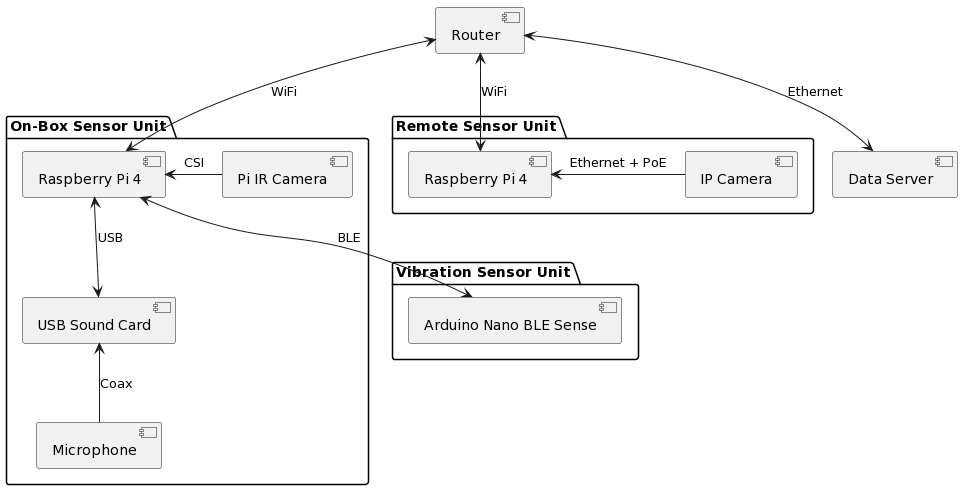
\includegraphics[width=0.8\textwidth]{images/System Diagram.png}
    \caption{System Diagram}
    \label{fig:sys_diag}
\end{figure}

For this to work, each major component is specified below.
\subsection{Data Server}
\begin{enumerate}
    \item The Data Server MUST aggregate all data from connected sensor nodes.
    \item The Data Server MUST provide an interface to access the aggregated data.
    \item The Data Server MUST add the following metadata to each data stream:
    \begin{enumerate}
        \item Originating sensor node
        \item Timestamp
    \end{enumerate}
    \item The Data Server MUST support nultiple sensor nodes that are dynamically added.
    \item The Data Server SHOULD support both encrypted and unencrypted sensor data.
    \item The Data Server SHOULD be capable of operating for 12 months without data offload or maintenance.
    \item The Data Server SHOULD be capable of automatically resuming operations after power loss.
\end{enumerate}
\subsection{On-Box Sensor Unit}
\begin{enumerate}
    \item The On-Box Sensor Unit MUST provide IR capable video data from the inside of the nesting box.
    \item The On-Box Sensor Unit MUST provide IR illumination when necessary.
    \item The On-Box Sensor Unit MUST provide audio data from the nesting box.
    \item The On-Box Sensor Unit SHOULD be capable of automatically resuming operations after power loss.
\end{enumerate}
\end{document}